  \documentclass[10pt]{article}

  \usepackage[utf8]{inputenc}
  \usepackage{floatrow}


  \usepackage{algorithm, algpseudocode}
  \let\oldReturn\Return
  \renewcommand{\Return}{\State\oldReturn}
  \newcommand{\N}{\mathbb{N}}
  \newcommand{\R}{\mathbb{R}}

  \usepackage[T1]{fontenc}
  \usepackage{enumitem}
  \usepackage{hyperref}
  \usepackage{graphicx}
  \usepackage{color}
  \usepackage{listings}
  \usepackage{wrapfig}
  \usepackage{amsmath}
  \usepackage{amsfonts}
  \usepackage{stmaryrd}
  \usepackage{mathtools}
  \usepackage[hmargin=1.25in,vmargin=1.25in]{geometry}
  \newcommand{\shellcmd}[1]{\\\indent\indent\texttt{\footnotesize\# #1}\\}
    
  %title setup
  \title{Projet informatique: Honshu (Lot C)}
  \author{
    Romain PEREIRA\\
    Douha OURIMI\\
    Afizullah RAHMANY\\
    Guangyue CHEN
  }
  \date{25/05/2018}

  % table of contents setup
  \renewcommand{\contentsname}{Sommaire}
  \usepackage{etoolbox}
  \patchcmd{\thebibliography}{\section*{\refname}}{}{}{}

  \hypersetup{
    colorlinks,
    citecolor=black,
    filecolor=black,
    linkcolor=blue,
    urlcolor=red
  }

  \begin{document}
    \maketitle
    \tableofcontents
    
    \newpage
    \section*{Préambule}
    Ce projet est réalisé dans le cadre de nos études à l'ENSIIE.
    L'objectif est de prendre en main des outils de 'programmation agile',
    en developpant un jeu de carte : le Honshu.
    \newline
    \begin{figure}[H]
      \begin{center}
	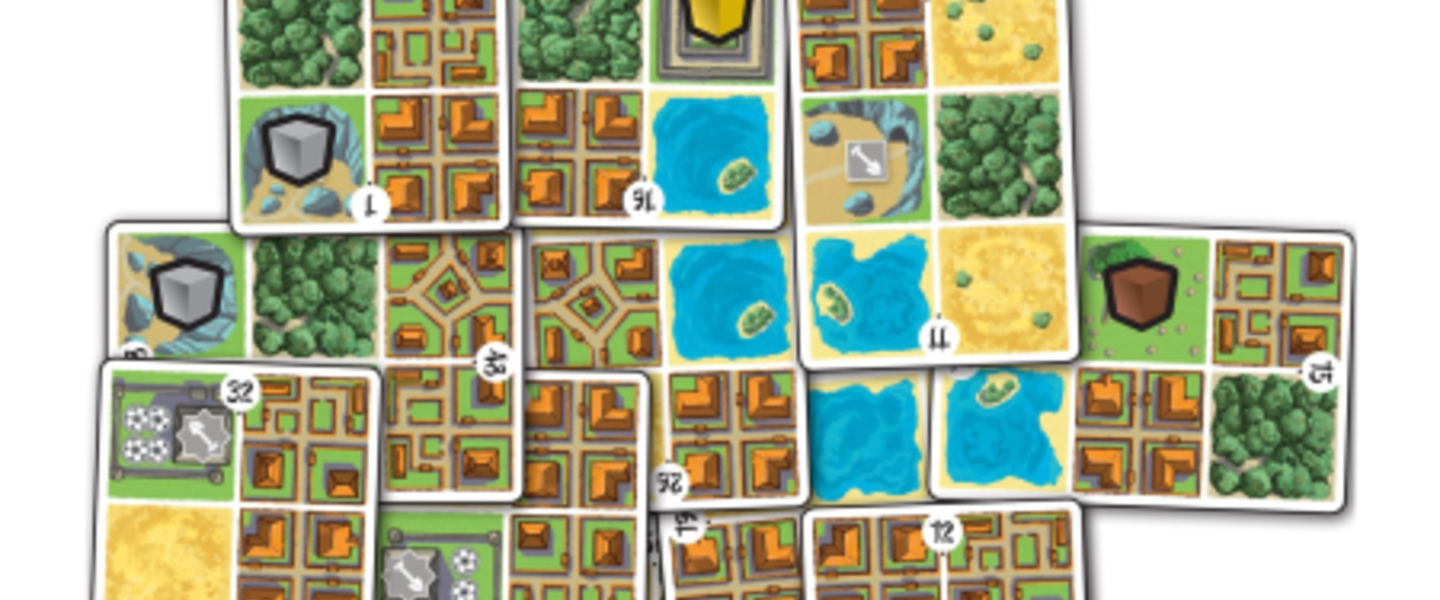
\includegraphics[height=6cm,keepaspectratio]{../images/honshu.png}
      \end{center}
      \caption{\textit{Plateau de jeu}}
      \label{honshu_introduction}
    \end{figure}
    \newpage
    \section{Introduction}
      Nous voici donc au lot D : Le jeu est fonctionnel et  s'affiche correctement à l'écran que ce soit en avec le terminale ou avec la librairie ncurses en affichage graphique.
      \newline Une partie se déroule jusqu'a son terme sans rencontrer de problème. Nous avons implémenter plusieurs solveurs nous donnant la meilleur manière de maximiser le score du joueur.
      \newline Dans ce dernier lot, il nous est demandé de rendre un jeu complet, avec la possibilité de soit permettre au joueur d'être capable de jouer à la souris ou de pouvoir lui laisser jouer avec des règles supplémentaire. 
      Nous avons opté pour la seconde option, dans la suite du rapport nous expliquerons comment nous avons offert la possibilité de modifier les règles.
      \newline Le travail a été séparé de la manière suivante :
      \newline
      \newline
      \textit{Douha} : implémentation des règles  : " Une plaine de quatre cases vaut 4 points (se rajoute) " et " Une case Lac vaut 2 points "
      \newline
      \newline
      \textit{Afizullah} : implémentation de la possibilité pour l'utilisateur d'ajouter des options lors du lancement de la partie.
      \newline
      \newline
      \textit{Romain} et \textit{Guangyue} :  implémentation des règles : "Une Usine peut accepter deux Ressources", "Un carré de quatre cases village, s’il est dans la ville comptabilisée, donne 4pts
  bonus" et "Pour chaque forêt, la première case vaut 1 point, la seconde 2 points, la troisième 3 points dans la limite de 5 etc.
  (max5)"
    \section{Modification de la présentation du jeu et implémentation des options}
      La Description fourni au lancement du jeu a été modfié pour également présenter les possibilité offertes à l'utilisateur concernant les règles supplémentaire applicables.
      \newline Pour ajouter de nouvelles option, nous avons compléter la fonction "getopt" avec les arguments -L -P - U - C -F correspondant chacune à une des nouvelles règles disponibles
      (voir 'main.c')
    \section{Implémentation des règles}
    Les nouvelles règles ont été implémenter à travers la modification de la fonction grille\_score.
    \lstset{language=C}          % Set your language (you can change the language for each code-block optionally)
    \begin{lstlisting}[frame=single]  % Start your code-block
switch (c->type) {
case TYPE_VILLE:

  village = grille_visit(grille, x, y, TYPE_VILLE);
  if (village > max_village) {
	  max_village = village;
  }
  break ;
  
case TYPE_LAC:

  if (FLAG_ISSET(flags, HS_RULE_LAC)) {
	  score += 2;
  } else {
	  score += 3 * (grille_visit(grille, x, y, TYPE_LAC) - 1);
    }
  break ;
  
case TYPE_FORET:

  if (FLAG_ISSET(flags, HS_RULE_FORET)) {
  nb_forets = grille_visit(grille, x, y, TYPE_FORET);
    if(nb_forets<=5) {
      score += nb_forets * (nb_forets + 1) / 2;
    } 
    else {
      score += (1 + 2 + 3 + 4 + 5) + 5 * (nb_forets - 5);
    }
  } 
  else {
    score += 2;
  }
  break ;
  
case TYPE_USINE:

  ++nb_usines;
  break;
  
case TYPE_RESSOURCE:

  ++nb_ressources;
  break ;
  
case TYPE_PLAINE:

  nb_plaines = grille_visit(grille, x, y, TYPE_PLAINE);
  if (FLAG_ISSET(flags, HS_RULE_PLAINE) && nb_plaines == 4) {
  score += 4;
  }
	break;
	
default:
	break ;
}
	

score += max_village;
score += MIN(FLAG_ISSET(flags, HS_RULE_FORET) ? 
nb_usines * 2 : nb_usines, nb_ressources) * 4;
return (score);
    \end{lstlisting}
    
      \newpage
    \section{Conclusion}
      Pour ce dernier lot, le travail a été séparé de manière efficace, et la plupart du code a ainsi pu être programmé pendant la séance encadré.
      Le jeu fonctionne comme espéré et le développement en méthode agile nous a permis de finir le projet dans les temps.
      
  \end{document}
